\subsection{Finding the iris with blob detection}
Our first approach to find the iris was to replicate the pupil detection method. By using different threshold values we tried to implement blob detection to find the center of the iris but this task was close to impossible. We found that the iris tended to either merge with other features, like eyelashes and pupil, or disintegrate into several components.
\begin{figure}[h]
	\centering
	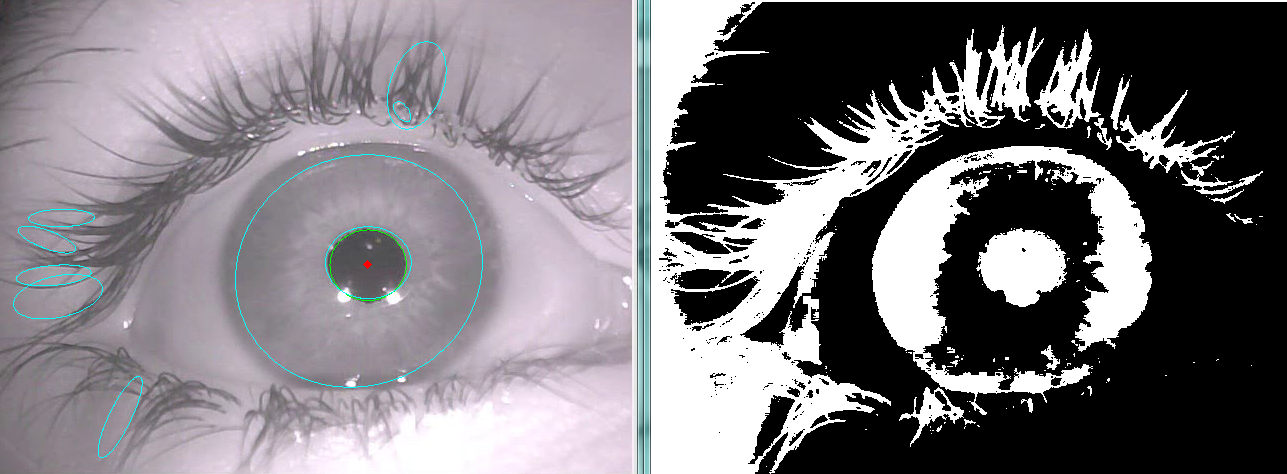
\includegraphics[scale=0.3]{iris_threshold_good.png}
	\caption{A rare instance where the iris is exactly identified.}
\end{figure}
\begin{figure}[h]
	\centering
	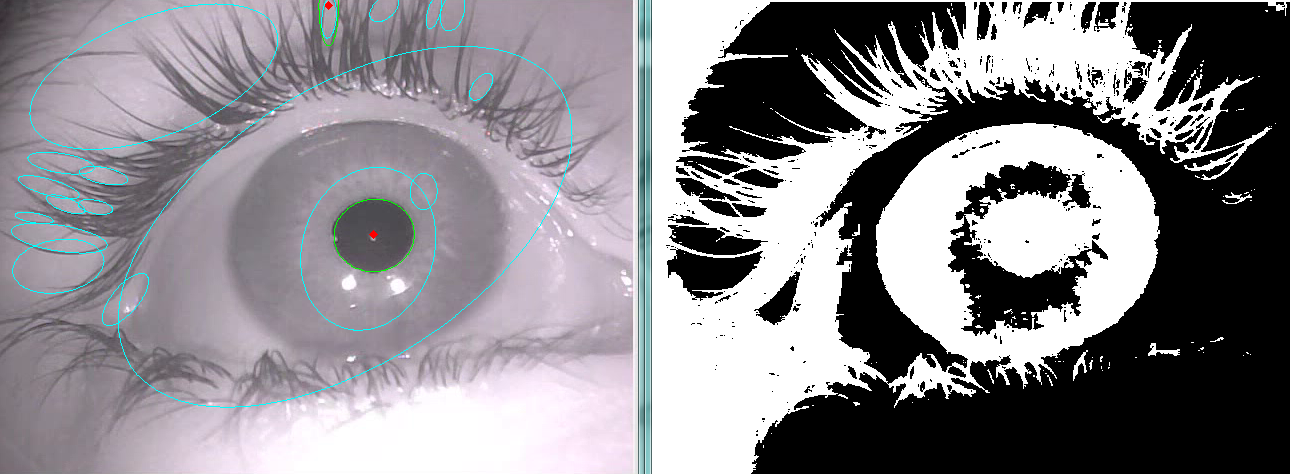
\includegraphics[scale=0.3]{iris_threshold_bad.png}
	\caption{A case where the iris is fused with its surrounding, yet still is not filled.}
\end{figure}
\newline
\subsection{Finding the iris with gradients} 
After the first approach failed we turned to gradients for iris detection. Boundaries in an image can be determined by a significant change of intensity between pixels. This change of intensity can be seen as a the slope, or gradient, at that point in the image. With this in mind we first calculated the gradients with respect to the x- and the y-dimensions. We then regarded these as coordinates of the gradient vector at each pixel, and used these to calculate the gradient magnitudes, and gradient directions. In general, the properties of these gradients where as expected. In areas where boundaries are present also grater gradients are present and their direction is towards the white area. \\
The edge of the iris was attempted found by finding the highest gradients along normals to a circle centered around the pupil. We fitted the length of these normals so that they generally stayed inside the eye, while not touching the pupil.\\
Even by trying to disregard pixels that where not aligned with the gradient curve the results where really affected by other features like the eyelashes.\\
The following figure shows the normals along which the highest gradient was identified. The blue lines are the normals along which gradients are found, and the blue orbs are the highest gradients along the line. The image shows that even with the entire iris boundary being located within the band searched, the edge detection still does not manage to find the boundary. The ellipse fitted to the points has little to do with the iris contour, and the edge detection generally seems happier locating the eyelashes and noisy detail in the iris than the softer boundary.
\begin{figure}[h]
	\centering
	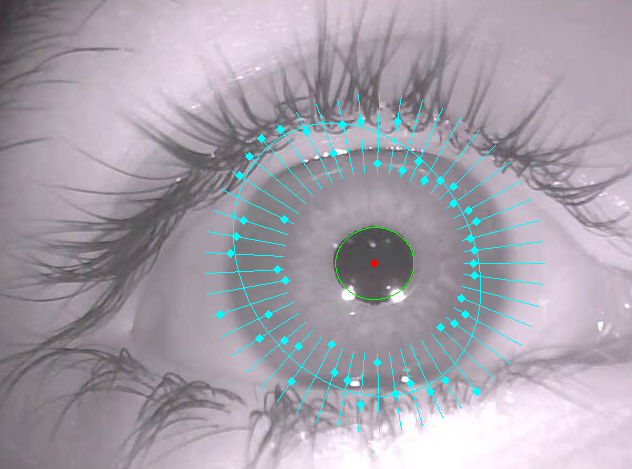
\includegraphics[scale=0.3]{iris_band_failure.png}
	\caption{The gradient along the normals failing to do their job.}
\end{figure}